\documentclass{beamer}
%
% Choose how your presentation looks.
%
% For more themes, color themes and font themes, see:
% http://deic.uab.es/~iblanes/beamer_gallery/index_by_theme.html
%
\mode<presentation>
{
  \usetheme{Madrid}      % or try Darmstadt, Madrid, Warsaw, ...
  \usecolortheme{whale} % or try albatross, beaver, crane, ...
  \usefonttheme{professionalfonts}  % or try serif, structurebold, ...
  \setbeamertemplate{navigation symbols}{}
  \setbeamertemplate{caption}[numbered]
} 

\usepackage[english]{babel}
\usepackage[utf8x]{inputenc}
\usepackage{multirow}
\usepackage{svg}
\usepackage{subcaption}



\title[Machine Learning and GPE]{Predicting energy expectation values for one-dimensional
non-linear Schrödinger Equation in random harmonic
potentials using artificial neural network}
\author{H{\"u}seyin Talha \c{S}enya\c{s}a\\090120132}
\institute{Advanced Physic Project Presentation}
%\date{\today}

\begin{document}

\begin{frame}
  \titlepage
\end{frame}

% Uncomment these lines for an automatically generated outline.
\begin{frame}{Outline}
  \tableofcontents
\end{frame}

\section{Machine Learning}

\subsection{Machine Learning}

\begin{frame}{Machine Learning}

$\bullet$ Artificial neural networks used in machine learning can approximate any continuous function within desired accuracy.

\vskip 1cm

$\bullet$ It is guaranteed that there exists
a network that satisfies the relation $|g(x) − f(x)| < \epsilon$.

\vskip 1cm

$\bullet$ Many different kind of applications of machine learning have already been implemented in physics.

%\begin{block}{Examples}
%Some examples of commonly used commands and features are included, to help you get started.
%\end{block}

\end{frame}


\begin{frame}{Machine Learning}

\begin{figure}[Htb!]
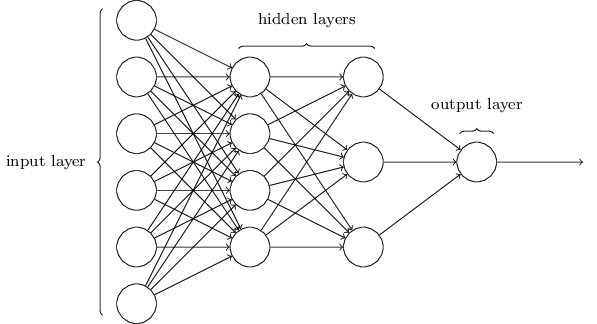
\includegraphics[width=0.6\textwidth]{neuralnetworkex.png}
\caption{\label{doppler_LP}An example of artificial neural network (Multi-layer perceptron)}
\end{figure}

\end{frame} 


\subsection{Deep Learning and Schr{\"o}dinger Equation}

\begin{frame}{Deep Learning and Schr{\"o}dinger Equation}

$\bullet$ Application of machine learning to a 2D Schr{\"o}dinger Equation with random potential.

\begin{figure}[Htb!]
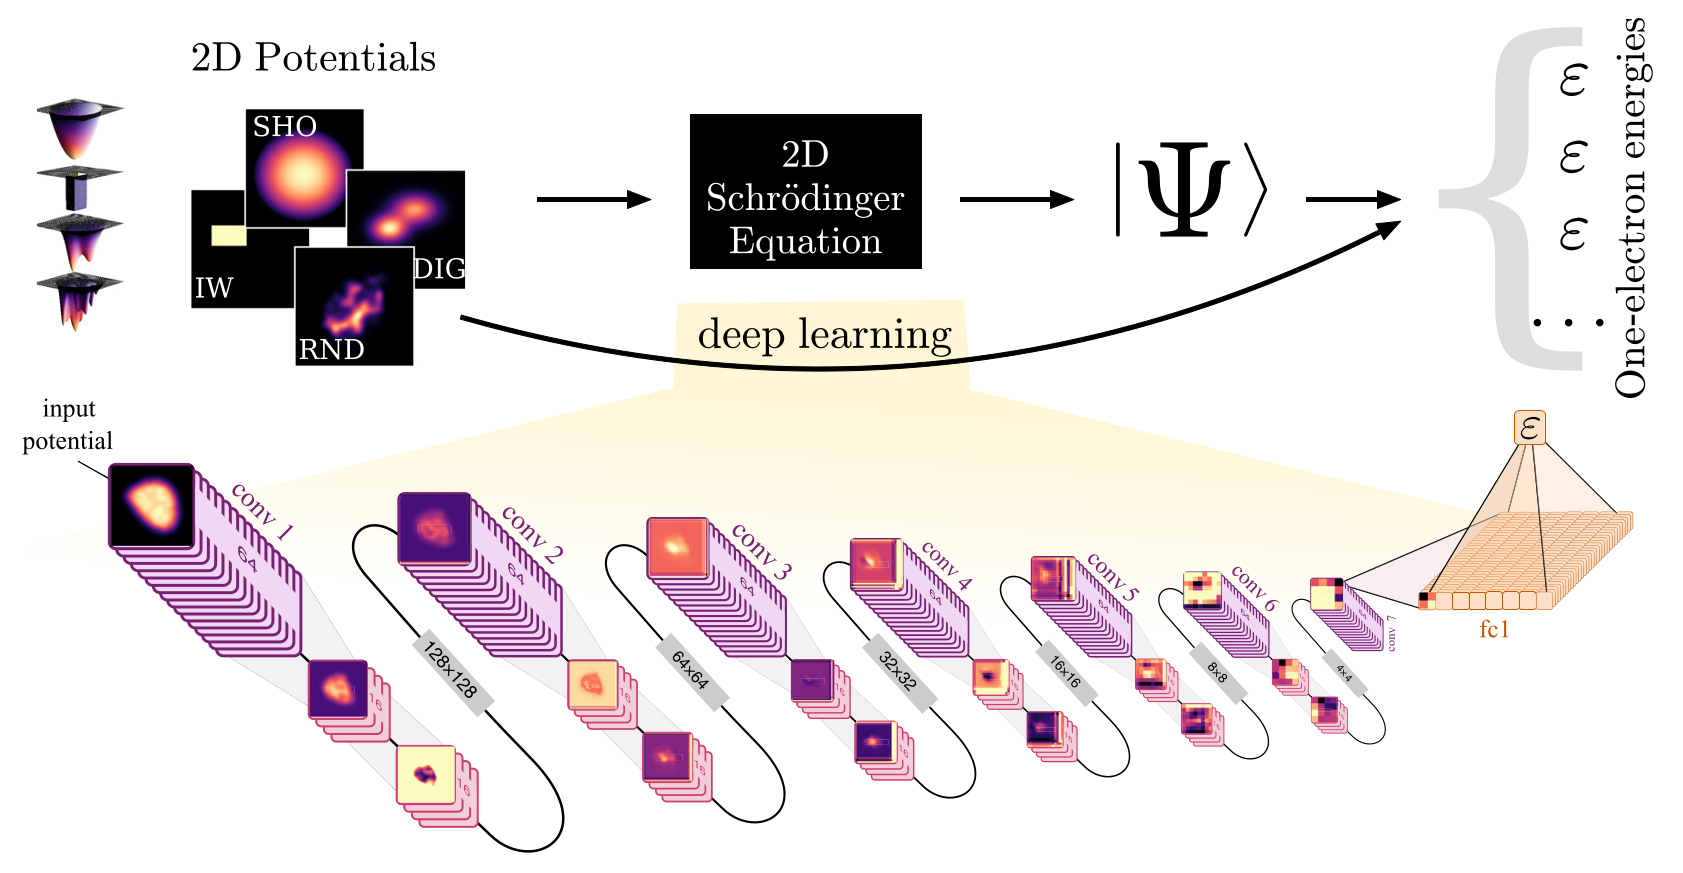
\includegraphics[width=0.8\textwidth]{DPandSE.png}
\caption{\label{fig:DPandSE} Deep Learning and Schr{\"o}dinger Equation.}
\end{figure}

\end{frame}

\begin{frame}{Deep Learning and Schr{\"o}dinger Equation}

$\bullet$ The article shows that a convolutional neural network can learn the mapping between $V(r)$ and physical features of the system.

\vskip 1cm

$\bullet$ It also shows that partial differential equations can be solved approximately with machine learning.

\end{frame}

\subsection{Applying Machine Learning to the NLSE}

\begin{frame}{Applying ML to the non-linear Schr{\"o}dinger Equation}

$$i \hbar \frac {\partial \Psi}{\partial t} = \frac {-\hbar^2}{2m}\nabla^2
\Psi + V(\boldsymbol{r}, t)\Psi + g|\Psi|^2\ \Psi$$

\vskip 0.5cm

$\bullet$ Gross-Pitaevskii Equation has non-linear term called as interaction parameter.

\vskip 0.5cm

$\bullet$ Interaction Parameter determines whether interaction is repulsive or attractive.

\vskip 0.5cm

$\bullet$ Analytic solutions are known for only few cases.

\vskip 0.5cm

$\bullet$ Generally solved by numerically or by approximation.


\end{frame}


\begin{frame}{Applying ML to the non-linear Schr{\"o}dinger Equation}

$\bullet$ GPE can also be studied in 1D

$$\mu^{\prime}\psi_z = \frac{-\hbar^2}{2m}\frac{d^2\psi_z}{dz^2} + \frac{1}{2}m\omega_z^2 (z-z_0)^2\psi_z + g^{\prime}|\psi_z|^2\psi_z$$

\begin{figure}[Htb!]
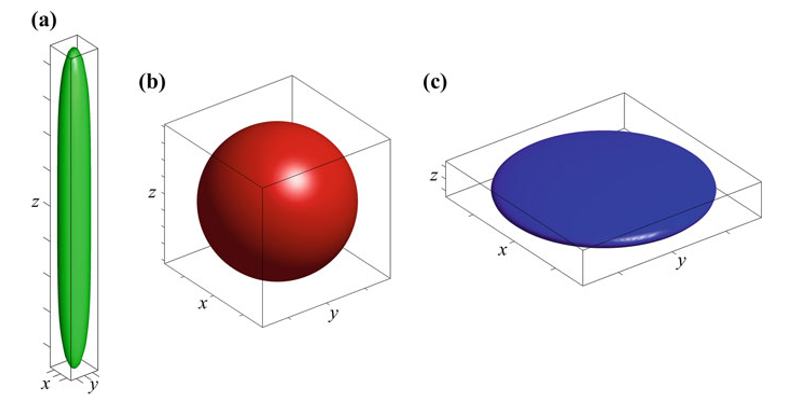
\includegraphics[width=0.8\textwidth]{BoseEinsteinCondensate.png}
\caption{\label{fig:DPandSE} Bose-Einstein Condensates in different trapping potentials.}
\end{figure}

\end{frame}

\section{Dataset Generation}
\subsection{Numerical Solution}

\begin{frame}{Numerical Solution}

$\bullet$ GPE is solved with random harmonic trapping potential including shift while interaction parameter is kept fixed.

\begin{table}[]
\centering
\caption{My caption}
\label{my-label}
\begin{tabular}{lllll}
Interaction Parameter & $g$\hspace{0.23cm}:       & \textbraceleft0, 0.1, 1, 10, 20\textbraceright &  &  \\
Shift                 & $z_0$\hspace{0.085cm}:     & {[}-5, 5{]}             &  &  \\
Angular Frequency     & $\omega_z$\hspace{0.05cm}:& {[}0.5, 2{]}            &  &  \\
                      &            &                         &  & 
\end{tabular}
\end{table}

$\bullet$ Solved by using imaginary time propagation and re-normalization in XMDS Framework.
\end{frame}

\begin{frame}{Numerical Solution}

%\svgpath{path = {"../../figs/dist/"}}
%\begin{figure}[H]
%    \centering
%    \begin{subfigure}[t]{0.45\textwidth}
%		%\centering
%        \includesvg[width=4cm]{energy-g-0-}
%        \caption{g = 0}
%		\label{fig:a}
%    \end{subfigure}
%    \begin{subfigure}[t]{0.45\textwidth}
%		%\centering
%        \includesvg[width=4cm]{energy-g-0_1-}
%        \caption{g = 0.1}
%		\label{fig:b}
%    \end{subfigure}
%    \begin{subfigure}[t]{0.45\textwidth}
%        %\centering
%        \includesvg[width=4cm]{energy-g-1-}
%        \caption{g = 1}
%		\label{fig:c}
%    \end{subfigure}
%    \begin{subfigure}[t]{0.45\textwidth}
%        %\centering
%        \includesvg[width=4cm]{energy-g-10-}
%        \caption{g = 10}
%		\label{fig:d}
%    \end{subfigure}
%    \caption{Total energy distributions of the generated solution for different interaction parameter values.}
%\label{fig:energy_dist}
%\end{figure}



%\svgpath{path = {"../../figs/dist/"}}
\begin{figure}[H]
	\includesvg[width=8cm]{potvsdens}
    \caption{Density}
	\label{fig:a}
\end{figure}

\end{frame}


\section{Neural Network}
\subsection{Neural Network}
\begin{frame}{Neural Network}

$\bullet$ Implemented in Pytorch Framework.\\
\vskip 0.5cm
$\bullet$ Two different neural network: Fully Connected, Convolutional.
\vskip 0.5cm
$\bullet$ Trained to predict ground state energy of a Bose-Einstein Condensate.
\vskip 0.5cm
$\bullet$ FCN is also trained to predict interaction, kinetic, potential, and total energy of the system.

\end{frame}

\begin{frame}{Fully Connected Network}

$\bullet$ 1 input layer, 3 hidden layers, 1 output layer.
\vskip 0.5cm
$\bullet$ Adaptive Learning Rate (Adam)
\vskip 0.5cm
$\bullet$ ReLU activation function

\end{frame}

\begin{frame}{Convolutional Neural Network}

$\bullet$ 2 convolution layers, 2 maxpool layers, 3 fully connected layer.
\vskip 0.5cm
$\bullet$ Adaptive Learning Rate (Adam)
\vskip 0.5cm
$\bullet$ ReLU activation function

\end{frame}

\begin{frame}{Choosing Hyperparameters}

\svgpath{path = {"../figs/archtestresults/"}}
\begin{figure}[H]
    \centering
    \begin{subfigure}[t]{0.45\textwidth}
           \centering
            \includesvg[width=\linewidth]{{"fourlayer-g0-lr0_003-800"}}
            \caption{FCN[128, 40, 40, 1], $\eta$ = 0.003}
            \label{fig:a}
    \end{subfigure}
    \begin{subfigure}[t]{0.45\textwidth}
            \centering
             \includesvg[width=\linewidth]{{"fourlayer-g0-lr0_001-800"}}
            \caption{FCN[128, 40, 40, 1], $\eta$ = 0.001}
            \label{fig:b}
    \end{subfigure}
    \caption{Hyperparameters}
\end{figure}
\end{frame}

\section{Training Results}
\subsection{Ground State Energy Predictions}

\begin{frame}{Ground State Energy Predictions}

\svgpath{path = {"../figs/FFN/"}}
\begin{figure}[H]
    \centering
    \begin{subfigure}[t]{0.45\textwidth}
		\centering
        \includesvg[width=4.5cm]{potential-g-0_1-epoch-20-}
		\label{fig:a}
    \end{subfigure}
    \begin{subfigure}[t]{0.45\textwidth}
		\centering
        \includesvg[width=4.5cm]{potential-g-0_1-epoch-40-}
		\label{fig:b}
    \end{subfigure}    
    \begin{subfigure}[t]{0.45\textwidth}
        \centering
        \includesvg[width=4.5cm]{potential-g-0_1-epoch-60-}
 		\label{fig:c}
    \end{subfigure}
    \begin{subfigure}[t]{0.45\textwidth}
        \centering
        \includesvg[width=4.5cm]{potential-g-0_1-epoch-60-LOSS-}
		\label{fig:c}
    \end{subfigure}
	{\caption{{FCN[128, 30, 30, 10, 1] results for $g = 0.1$.}}}
\label{fig:FFN-g-0.1}
\end{figure}

\end{frame}


\begin{frame}{Ground State Energy Predictions}

\svgpath{path = {"../figs/CNN/"}}
\begin{figure}[H]
    \centering
    \begin{subfigure}[t]{0.45\textwidth}
		\centering
        \includesvg[width=4.5cm]{potential-g-1-conv1d-epoch-20-}
		\label{fig:a}
    \end{subfigure}
    \begin{subfigure}[t]{0.45\textwidth}
		\centering
        \includesvg[width=4.5cm]{potential-g-1-conv1d-epoch-40-}
		\label{fig:b}
    \end{subfigure}    
    \begin{subfigure}[t]{0.45\textwidth}
        \centering
        \includesvg[width=4.5cm]{potential-g-1-conv1d-epoch-60-}
		\label{fig:c}
    \end{subfigure}
    \begin{subfigure}[t]{0.45\textwidth}
        \centering
        \includesvg[width=4.5cm]{potential-g-1-conv1d-epoch-60-LOSS-}
		\label{fig:c}
    \end{subfigure}
	\caption{CNN results for $g = 1$}
\label{fig:CNN-g-1}
\end{figure}

\end{frame}

\begin{frame}{Ground State Energy Predictions}

\svgpath{path = {"../figs/FFNMERGED/"}}
\begin{figure}[H]
    \centering
    \begin{subfigure}[t]{0.45\textwidth}
		\centering
        \includesvg[width=4.5cm]{potential-g-1-epoch-60-E_int-}
		\label{fig:a}
    \end{subfigure}
    \begin{subfigure}[t]{0.45\textwidth}
		\centering
        \includesvg[width=4.5cm]{potential-g-1-epoch-60-E_pot-}
		\label{fig:b}
    \end{subfigure}    
    \begin{subfigure}[t]{0.45\textwidth}
        \centering
        \includesvg[width=4.5cm]{potential-g-1-epoch-60-E_kin-}
		\label{fig:c}
    \end{subfigure}
    \begin{subfigure}[t]{0.45\textwidth}
        \centering
        \includesvg[width=4.5cm]{potential-g-1-epoch-60-E_Total-}
		\label{fig:c}
    \end{subfigure}
	\caption{FCN[128, 30, 30, 10, 4], Separate energy predictions for $g = 1$.}
\label{fig:FFN-g-1-S}
\end{figure}
\end{frame}

\subsection{Predicting Interaction Parameter}
\begin{frame}{Inverse Problem: Predicting interaction parameter}

\svgpath{path = {"../figs/CNNgPrediction/"}}
\begin{figure}[H]
    \centering
    \begin{subfigure}[t]{0.45\textwidth}
		\centering
    	\includesvg[width=4.5cm]{fixed-pot_dens-g-VARY-conv1d-epoch-30-}
		\label{fig:a}
    \end{subfigure}
    \begin{subfigure}[t]{0.45\textwidth}
        \centering
    	\includesvg[width=4.5cm]{various-pot_dens-g-VARY-conv1d-epoch-30-}
		\label{fig:b}
    \end{subfigure}
    \begin{subfigure}[t]{0.45\textwidth}
        \centering
		\includesvg[width=4.5cm]{various-shift-pot_dens-g-VARY-conv1d-epoch-30-}
		\label{fig:c}
    \end{subfigure}
    \begin{subfigure}[t]{0.45\textwidth}
        \centering
		\includesvg[width=4.5cm]{FPFS-VPFS-VPVS-LOSS-}
		\label{fig:d}
    \end{subfigure}
\end{figure}
\end{frame}

\end{document}
